%%%%%%%%%%%%%%%%%%%%%%%%%%%%%%%%%%%%%%%%%%%%%%%%%%%%%%%%%%%%%%%%%
% MUW Presentation
% LaTeX Template
% Version 1.0 (27/12/2016)
%
% License:
% CC BY-NC-SA 4.0 (http://creativecommons.org/licenses/by-nc-sa/3.0/)
%
% Created by:
% Nicolas Ballarini, CeMSIIS, Medical University of Vienna
% nicoballarini@gmail.com
% http://statistics.msi.meduniwien.ac.at/
%
% Customized for UAH by:
% David F. Barrero, Departamento de Automática, UAH
%%%%%%%%%%%%%%%%%%%%%%%%%%%%%%%%%%%%%%%%%%%%%%%%%%%%%%%%%%%%%%%%%

\documentclass[10pt,compress]{beamer} % Change 10pt to make fonts of a different size
\mode<presentation>

\usepackage[spanish]{babel}
\usepackage{fontspec}
\usepackage{tikz}
\usepackage{etoolbox}
\usepackage{xcolor}
\usepackage{xstring}
\usepackage{listings}

% Custom packages
\usepackage{tikz}
\usepackage{standalone}
\def\layersep{2.5cm}
\usetikzlibrary{matrix,chains,positioning,decorations.pathreplacing,arrows,tikzmark}

\usetheme{UAH}
\usecolortheme{UAH}
\setbeamertemplate{navigation symbols}{} 
\setbeamertemplate{caption}[numbered]

%%%%%%%%%%%%%%%%%%%%%%%%%%%%%%%%%%%%%%%%%%%%%%%%%%%%%%%%%%%%%%%%%
%% Presentation Info
\title[Neuroevolution]{Neuroevolution}
\author{}
\institute{\asignatura}
\date{}
%%%%%%%%%%%%%%%%%%%%%%%%%%%%%%%%%%%%%%%%%%%%%%%%%%%%%%%%%%%%%%%%%


%%%%%%%%%%%%%%%%%%%%%%%%%%%%%%%%%%%%%%%%%%%%%%%%%%%%%%%%%%%%%%%%%
%% Descomentar para habilitar barra de navegación superior
\setNavigation
%%%%%%%%%%%%%%%%%%%%%%%%%%%%%%%%%%%%%%%%%%%%%%%%%%%%%%%%%%%%%%%%%

%%%%%%%%%%%%%%%%%%%%%%%%%%%%%%%%%%%%%%%%%%%%%%%%%%%%%%%%%%%%%%%%%
%% Configuración de logotipos en portada
%% Opacidad de los logotipos
\newcommand{\opacidad}{1}
%% Descomentar para habilitar logotipo en pié de página de portada
\renewcommand{\logoUno}{Images/isg.png}
%% Descomentar para habilitar logotipo en pié de página de portada
%\renewcommand{\logoDos}{Images/CCLogo.png}
%% Descomentar para habilitar logotipo en pié de página de portada
%\renewcommand{\logoTres}{Images/ALogo.png}
%% Descomentar para habilitar logotipo en pié de página de portada
%\renewcommand{\logoCuatro}{Images/ELogo.png}
%%%%%%%%%%%%%%%%%%%%%%%%%%%%%%%%%%%%%%%%%%%%%%%%%%%%%%%%%%%%%%%%%

%%%%%%%%%%%%%%%%%%%%%%%%%%%%%%%%%%%%%%%%%%%%%%%%%%%%%%%%%%%%%%%%%
%% FOOTLINE
%% Comment/Uncomment the following blocks to modify the footline
%% content in the body slides. 


%% Option A: Title and institute
\footlineA
%% Option B: Author and institute
%\footlineB
%% Option C: Title, Author and institute
%\footlineC
%%%%%%%%%%%%%%%%%%%%%%%%%%%%%%%%%%%%%%%%%%%%%%%%%%%%%%%%%%%%%%%%%

\begin{document}

%%%%%%%%%%%%%%%%%%%%%%%%%%%%%%%%%%%%%%%%%%%%%%%%%%%%%%%%%%%%%%%%%
% Use this block for a blue title slide with modified footline
{\titlepageBlue
    \begin{frame}
        \titlepage
    \end{frame}
}

\begin{frame}[plain]{}
   \begin{block}{Objective}
      \begin{itemize}
        \item Fusion ANN and Evolutionary Algorithms
        \item Identify application areas of Neuroevolution in Robotics
      \end{itemize}
   \end{block}

   \begin{block}{Bibliography}
      \begin{enumerate}
        \item A. Tettamanzi, M. Tomassini. \textit{Soft Computing. Integrating Evolutionary, Neural, and Fuzzy Systems}. Springer-Verlag. 2001
        \item D. Floreano, P. D\"urr, C. Mattiussi. \textit{Neuroevolution: from architectures to learning}. Evolutionary Intelligence, Vol. 1, No. 1, pags. 47-62. Springer-Verlag. 2008.
        \item S. Risi, J. Togelius. \textit{Neuroevolution in Games: State of the Art and Open Challenges}. IEEE Trans. on Computational Intelligence and AI in Games. Vol 9, No. 1. 2017
      \end{enumerate} 
   \end{block}
\end{frame}

{
\disableNavigation{white}
\begin{frame}[shrink]{Table of Contents}
 \frametitle{Table of Contents}
 \tableofcontents
  % You might wish to add the option [pausesections]
\end{frame}
}

\section{Introduction}
\subsection{Motivation}
\begin{frame}{Introduction}{Motivation}
	Problems with traditional learning algorithms
	\begin{itemize}
        \item Fixed topology
        \item Local mimina and other learning limitations
	\end{itemize}
	In Nature ...
	\begin{itemize}
        \item Global neural system architecture given by evolution
        \item Details (synapsys) given by learning
	\end{itemize}
    EAs good avoiding local maxima and searching complex search spaces
\end{frame}

\subsection{Definition}
\begin{frame}{Introduction}{Definition (I)}
    \begin{columns}
 	   \column{.80\textwidth}
       \vspace{-0.3cm}
       \begin{block}{Neuroevolution (NE)}
            \textit{NE refers to the generation of artificial neural networks (their connections weights and/or topology) using evolutionary algorithms}

            \vspace{-0.2cm}
            \begin{flushright} Risi and Togelius\end{flushright}
        \end{block}
    \end{columns}

    NE features
	\begin{itemize}
        \item Record-beating performance
        \item Broad applicability
        \item Scalability
        \item Diversity
        \item Open-ended learning
	\end{itemize}
    Problem: NE does not provide explicative models
\end{frame}

\begin{frame}{Introduction}{Definition (II)}
    When ANN meets EAs
	\begin{itemize}
        \item Evolve weights
        \item Evolve topology
	\end{itemize}
    Key elements to take into account
	\begin{itemize}
        \item Evaluation (straight or hybrid) (not accepted terms)
        \item Representation (direct or indirect)
	\end{itemize}
\end{frame}

\section{ANN evaluation}

\subsection{Straight approach}

\begin{frame}{ANN evaluation}{Straight approach}
	Straight: Build ANN and assess it
   		\begin{itemize}
		\item Cumulative error on test set
		\item Simulate robot behavior
		\item Observe robot behavior
   		\end{itemize}
	Some problems
		\begin{itemize}
		\item Pretty slow
		\item Does not explot gradient if available
		\end{itemize}
\end{frame}

\subsection{Hybrid approach}

\begin{frame}{ANN evaluation}{Hybrid approach}
	Hybrid: Join evolution and learning
	\begin{itemize}
		\item EAs have good exploration
		\item Training has good explotation
		\item Gradient-based methods sensible to initial weights
	\end{itemize}
	Evolve a population of ANN, then train them (backprop, ...)
	\begin{itemize}
		\item Trainning does not change genotype
    \end{itemize}

	\begin{center}
	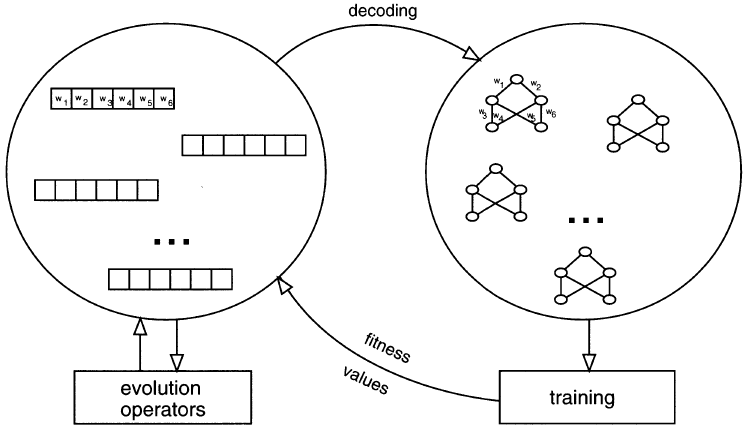
\includegraphics[width=0.4\linewidth]{figs/hybrid.png}\\
    \tiny{A. Tettamanzi, M. Tomassini. \textit{Soft Computing. Integrating Evolutionary, Neural, and Fuzzy Systems}. Springer-Verlag. 2001}
	\end{center}
\end{frame}



\section{Direct codification}
\subsection{Direct codification of ANNs}

\begin{frame}{Direct codification}{Direct codification of ANNs}
    \begin{columns}
 	   \column{.50\textwidth}
        Each gene represents a weight
	        \begin{itemize}
                \item Fixed topology
	        \end{itemize}
        Can be used any EA
	        \begin{itemize}
                \item Typically, GA or ES
	        \end{itemize}
        Several complex neuroevolution specific codifications
 	    \column{.50\textwidth}
            \documentclass{standalone}
\usepackage{tikz}

\usetikzlibrary{positioning,arrows}

\begin{document}
\begin{tikzpicture}[shorten >=1pt,->,draw=black!50, node distance=\layersep]
    \tikzstyle{every pin edge}=[<-,shorten <=1pt]
	\tikzstyle{neuron}=[circle,draw=black!75,minimum size=17pt,inner sep=0pt]
	\tikzstyle{input neuron}=[neuron];
	\tikzstyle{output neuron}=[neuron];
	\tikzstyle{hidden neuron}=[neuron];
	\tikzstyle{annot} = [midway, left, font=\scriptsize]
    \tikzstyle{edge} = [->, >=latex']

    \node[output neuron] (output) at (0, 2.5) {};
    \node[hidden neuron] (hiddenL) at (-1, 1.5) {};
    \node[hidden neuron] (hiddenR) at (1, 1.5) {};
    \node[input neuron] (inputL) at (-1, 0) {};
    \node[input neuron] (inputR) at (1, 0) {};

    \draw[edge] (hiddenL) edge node [annot] {$0.2$} (output);
    \draw[edge] (hiddenR) edge node [annot, right] {$-0.3$} (output);

    \draw[edge] (inputL) edge node [annot] {$0.6$} (hiddenL);
    \draw[edge] (inputL) edge node [annot, pos=0.3] {$-0.5$} (hiddenR);

    \draw[edge] (inputR) edge node [annot, pos=0.3, right] {$0.4$} (hiddenL);
    \draw[edge] (inputR) edge node [annot, right] {$0.7$} (hiddenR);

    \node (chromosome) at (0, -1) {(0.2, -0.3, 0.6, -0.5, 0.4, 0.7)};

	%\node[input neuron, pin=left:Input \#\y] (I-\name) at (0,-\y) {};
	%node[hidden neuron] (H-\name) at (\layersep,-\y cm) {}; 
	% Draw the output layer node 
	%\node[output neuron,pin={[pin edge={->}]right:Output}, right of=H-3] (O) {}; 
	% Connect every node in the input layer with every node in the 
	% hidden layer. 
	% Connect every node in the hidden layer with the output layer 
	% Annotate the layers 
	%\node[annot,above of=H-1, node distance=1cm] (hl) {Hidden layer}; 
	%\node[annot,left of=hl] {Input layer}; 
	%\node[annot,right of=hl] {Output layer};
\end{tikzpicture}
\end{document}

    \end{columns}
\end{frame}

\subsection{Alternative direct codification of ANNs}

\begin{frame}{Direct codification}{Alternative direct codification of ANNs}
    \tikzstyle{every picture}+=[remember picture]
    \begin{columns}
 	   \column{.50\textwidth}
      \documentclass{standalone}
\usepackage{tikz}

\usetikzlibrary{positioning,arrows}

\begin{document}
\begin{tikzpicture}[shorten >=1pt,->,draw=black!50, node distance=\layersep]
    \tikzstyle{every pin edge}=[<-,shorten <=1pt]
	\tikzstyle{neuron}=[circle,draw=black!75,minimum size=17pt,inner sep=0pt]
	\tikzstyle{input neuron}=[neuron];
	\tikzstyle{output neuron}=[neuron];
	\tikzstyle{hidden neuron}=[neuron];
	\tikzstyle{annot} = [midway, left, font=\scriptsize]
    \tikzstyle{edge} = [->, >=latex']

    \node[output neuron] (output) at (0, 3) {6};
    \node[hidden neuron] (hiddenL) at (-1, 1.5) {4};
    \node[hidden neuron] (hiddenR) at (1, 1.5) {5};
    \node[input neuron] (inputL) at (-2, 0) {1};
    \node[input neuron] (inputC) at (0, 0) {2};
    \node[input neuron] (inputR) at (2, 0) {3};

    \draw[edge] (hiddenR) edge (output);
    \draw[edge] (hiddenL) edge (output);

    \draw[edge] (inputR) edge (hiddenR);
    \draw[edge] (inputL) edge (hiddenL);
    \path (inputL) -- coordinate (aux14) (hiddenL);
    \draw[edge] (inputL) edge (hiddenR);
    \path (inputL) -- coordinate (aux15) (hiddenR);

    \draw[edge] (inputC) edge (output);
    \draw[edge] (inputC) edge (hiddenL);

    %\node (chromosome) at (0, -1) {(-0.3, 0.2, 0.7, 0.4, -0.5, 0.6)};

	%\node[input neuron, pin=left:Input \#\y] (I-\name) at (0,-\y) {};
	%node[hidden neuron] (H-\name) at (\layersep,-\y cm) {}; 
	% Draw the output layer node 
	%\node[output neuron,pin={[pin edge={->}]right:Output}, right of=H-3] (O) {}; 
	% Connect every node in the input layer with every node in the 
	% hidden layer. 
	% Connect every node in the hidden layer with the output layer 
	% Annotate the layers 
	%\node[annot,above of=H-1, node distance=1cm] (hl) {Hidden layer}; 
	%\node[annot,left of=hl] {Input layer}; 
	%\node[annot,right of=hl] {Output layer};
\end{tikzpicture}
\end{document}


 	   \column{.50\textwidth}

        \begin{table}[]
            \centering
                \begin{tabular}{l|llllll}
                 & 1 & 2 & 3 & 4 & 5 & 6 \\\hline
               1 & 0 & 0 & 0 & \tikzmark{four}1 & \tikzmark{five}1 & 0 \\
               2 & 0 & 0 & 0 & 1 & 0 & 1 \\
               3 & 0 & 0 & 0 & 0 & 1 & 0 \\
               4 & 0 & 0 & 0 & 0 & 0 & 1 \\
               5 & 0 & 0 & 0 & 0 & 0 & 1 \\
               6 & 0 & 0 & 0 & 0 & 0 & 0
                \end{tabular}
         \end{table}

    \begin{tikzpicture}[overlay, remember picture]
         \draw <2-> [->, blue!50, in=90, out=120] ({pic cs:four}) to (aux14);
         \draw <2-> [->, blue!50, in=90, out=120] ({pic cs:five}) to (aux15);
    \end{tikzpicture}

    \end{columns}
\end{frame}

\subsection{Permutation problem}

\begin{frame}{Direct codification}{Permutation problem}
     Permutation problem (also known as compeling convenions)
	 \begin{itemize}
        \item Multiple genotypes with same phenotype
	 \end{itemize}

     \documentclass{standalone}
\usepackage{tikz}

\usetikzlibrary{positioning,arrows}

\begin{document}
\begin{tikzpicture}[shorten >=1pt,->,draw=black!50, node distance=\layersep]
    \tikzstyle{every pin edge}=[<-,shorten <=1pt]
	\tikzstyle{neuron}=[circle,draw=black!75,minimum size=17pt,inner sep=0pt]
	\tikzstyle{input neuron}=[neuron];
	\tikzstyle{output neuron}=[neuron];
	\tikzstyle{hidden neuron}=[neuron];
	\tikzstyle{annot} = [midway, left, font=\scriptsize]
    \tikzstyle{edge} = [->, >=latex']

    \node[output neuron] (output) at (0, 2.5) {};
    \node[hidden neuron] (hiddenL) at (-1, 1.5) {};
    \node[hidden neuron] (hiddenR) at (1, 1.5) {};
    \node[input neuron] (inputL) at (-1, 0) {};
    \node[input neuron] (inputR) at (1, 0) {};

    \draw[edge] (hiddenL) edge node [annot] {$0.2$} (output);
    \draw[edge] (hiddenR) edge node [annot, right] {$-0.3$} (output);

    \draw[edge] (inputL) edge node [annot] {$0.6$} (hiddenL);
    \draw[edge] (inputL) edge node [annot, pos=0.3] {$-0.5$} (hiddenR);

    \draw[edge] (inputR) edge node [annot, pos=0.3, right] {$0.4$} (hiddenL);
    \draw[edge] (inputR) edge node [annot, right] {$0.7$} (hiddenR);

    \node (chromosome) at (0, -1) {(0.2, -0.3, 0.6, -0.5, 0.4, 0.7)};

	%\node[input neuron, pin=left:Input \#\y] (I-\name) at (0,-\y) {};
	%node[hidden neuron] (H-\name) at (\layersep,-\y cm) {}; 
	% Draw the output layer node 
	%\node[output neuron,pin={[pin edge={->}]right:Output}, right of=H-3] (O) {}; 
	% Connect every node in the input layer with every node in the 
	% hidden layer. 
	% Connect every node in the hidden layer with the output layer 
	% Annotate the layers 
	%\node[annot,above of=H-1, node distance=1cm] (hl) {Hidden layer}; 
	%\node[annot,left of=hl] {Input layer}; 
	%\node[annot,right of=hl] {Output layer};
\end{tikzpicture}
\end{document}
 
     \documentclass{standalone}
\usepackage{tikz}

\usetikzlibrary{positioning,arrows}

\begin{document}
\begin{tikzpicture}[shorten >=1pt,->,draw=black!50, node distance=\layersep]
    \tikzstyle{every pin edge}=[<-,shorten <=1pt]
	\tikzstyle{neuron}=[circle,draw=black!75,minimum size=17pt,inner sep=0pt]
	\tikzstyle{input neuron}=[neuron];
	\tikzstyle{output neuron}=[neuron];
	\tikzstyle{hidden neuron}=[neuron];
	\tikzstyle{annot} = [midway, left, font=\scriptsize]
    \tikzstyle{edge} = [->, >=latex']

    \node[output neuron] (output) at (0, 2.5) {};
    \node[hidden neuron] (hiddenL) at (-1, 1.5) {};
    \node[hidden neuron] (hiddenR) at (1, 1.5) {};
    \node[input neuron] (inputL) at (-1, 0) {};
    \node[input neuron] (inputR) at (1, 0) {};

    \draw[edge] (hiddenR) edge node [annot,right] {$0.2$} (output);
    \draw[edge] (hiddenL) edge node [annot] {$-0.3$} (output);

    \draw[edge] (inputR) edge node [annot,right] {$0.6$} (hiddenR);
    \draw[edge] (inputR) edge node [annot, pos=0.3,right] {$-0.5$} (hiddenL);

    \draw[edge] (inputL) edge node [annot, left] {$0.7$} (hiddenL);
    \draw[edge] (inputL) edge node [annot, pos=0.3,left] {$0.4$} (hiddenR);

    \node (chromosome) at (0, -1) {(-0.3, 0.2, 0.7, 0.4, -0.5, 0.6)};

	%\node[input neuron, pin=left:Input \#\y] (I-\name) at (0,-\y) {};
	%node[hidden neuron] (H-\name) at (\layersep,-\y cm) {}; 
	% Draw the output layer node 
	%\node[output neuron,pin={[pin edge={->}]right:Output}, right of=H-3] (O) {}; 
	% Connect every node in the input layer with every node in the 
	% hidden layer. 
	% Connect every node in the hidden layer with the output layer 
	% Annotate the layers 
	%\node[annot,above of=H-1, node distance=1cm] (hl) {Hidden layer}; 
	%\node[annot,left of=hl] {Input layer}; 
	%\node[annot,right of=hl] {Output layer};
\end{tikzpicture}
\end{document}

\end{frame}

\subsection{Symbolic, adaptive, neuro-evolution (SANE)}
\begin{frame}{Direct codification}{Symbolic, adaptive, neuro-evolution (SANE)}
    \begin{columns}
 	   \column{.50\textwidth}
		SANE evolves single neurons
		\begin{itemize}
			\item Population of neurons
			\item Connections and weights
			\item Fixed topology: One hidden layer
		\end{itemize}
 	   \column{.50\textwidth}
		Evaluation
		\begin{enumerate}
			\item Build random ANNs with sampled neurons
			\item Compute ANNs fitness
			\item Fitness of a neuron is the average fitness of all the ANNs it has participated in
		\end{enumerate}
	\end{columns}
		\begin{center}
		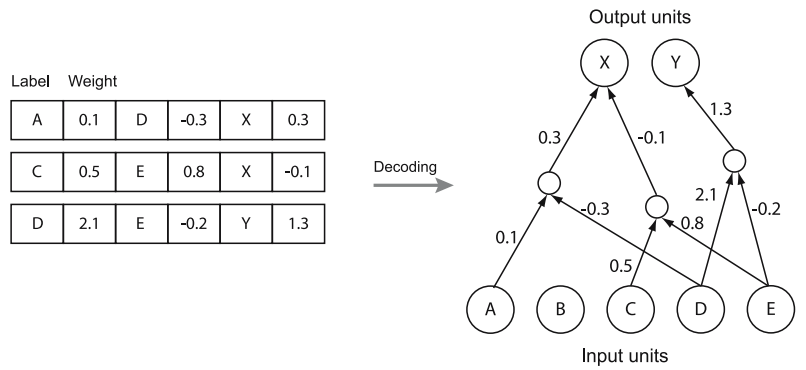
\includegraphics[width=0.5\linewidth]{figs/sane.png}\\
    	\tiny{ D. Floreano, P. D\"urr, C. Mattiussi. \textit{Neuroevolution: from architectures to learning}. Evolutionary Intelligence, Vol. 1, No. 1, pags. 47-62. Springer-Verlag. 2008.}
		\end{center}
\end{frame}

\subsection{Neuro-evolution of Augmenting Topologies (NEAT)}
\begin{frame}{Direct codification}{Neuro-evolution of Augmenting Topologies (NEAT)}
    \begin{columns}
 	   \column{.50\textwidth}
	Quite used NE algorithm
	\begin{itemize}
		\item Weights and \textit{topologies}
		\item Grows ANN complexity
	\end{itemize}
	Two types of genes
	\begin{itemize}
		\item Nodes and connections
	\end{itemize}
	Genetic operators
	\begin{itemize}
		\item Meaningful crossover
		\item Gene enable/disable mutation
		\item Gene insert operator
	\end{itemize}
	\href{https://www.youtube.com/watch?v=3JiNC6vw8zE}{(Video Torcs)}
	\href{https://www.youtube.com/watch?v=tmltm0ZHkHw}{(Video Mario)}
 	\column{.50\textwidth}
	\begin{center}
	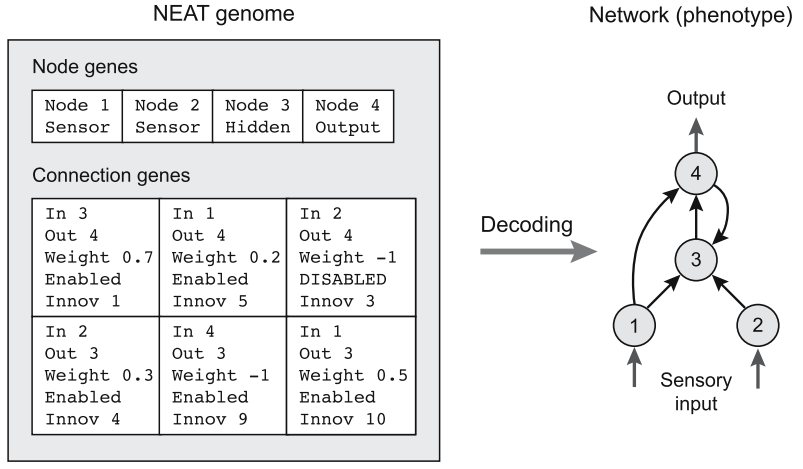
\includegraphics[width=\linewidth]{figs/neat.png}\\
    \tiny{ D. Floreano, P. D\"urr, C. Mattiussi. \textit{Neuroevolution: from architectures to learning}. Evolutionary Intelligence, Vol. 1, No. 1, pags. 47-62. Springer-Verlag. 2008.}
	\end{center}
	\end{columns}
\end{frame}

%\subsection{Covariance Matrix Adaptation (CMA-ES)}

\section{Indirect codification}

\subsection{Introduction}
\begin{frame}{Indirect codification}{Introduction}
	Problems with direct codification
	\begin{itemize}
		\item Scalability
		\item No reuse
	\end{itemize}
	Indirect encoding try to grow networks
	\begin{itemize}
		\item Evolve generation rules instead of individual weights
		\item Try to reuse basic building blocks
		\item Closer to biological systems
	\end{itemize}
\end{frame}

\subsection{Kitano's method}

\begin{frame}[fragile]{Indirect codification}{Kitano's method (I)}
    \begin{columns}
 	   \column{.40\textwidth}
	   Kitano used rewriting rules
	   \begin{itemize}
	   	\item Terminals, a symbol 
		\item Non-terminals, a rewriting rule
	   \end{itemize}

 	   \column{.60\textwidth}
	   		\begin{exampleblock}{Grammar example}
				\small{
				\texttt{
				<digit> $\longrightarrow$ 0|1|2|3|4|5|6|7|8|9\\
				<number> $\longrightarrow$ <digit>\\
				<number> $\longrightarrow$ <number><digit>}
				}
			\end{exampleblock}
    \end{columns}

	\bigskip
	Rather standard GA evolve rules
	\begin{itemize}
		\item Fitness proportionale, elitism, variable mutation rate, single crossover
		\item Evaluation of the network trained with backpropagation
	\end{itemize}

	Cromosomes composed by
	\begin{itemize}
		\item Fixed and evolvable rules
	\end{itemize}

\end{frame}

\begin{frame}[plain]{Indirect codification}{Kitano's method (II)}
	\begin{center}
	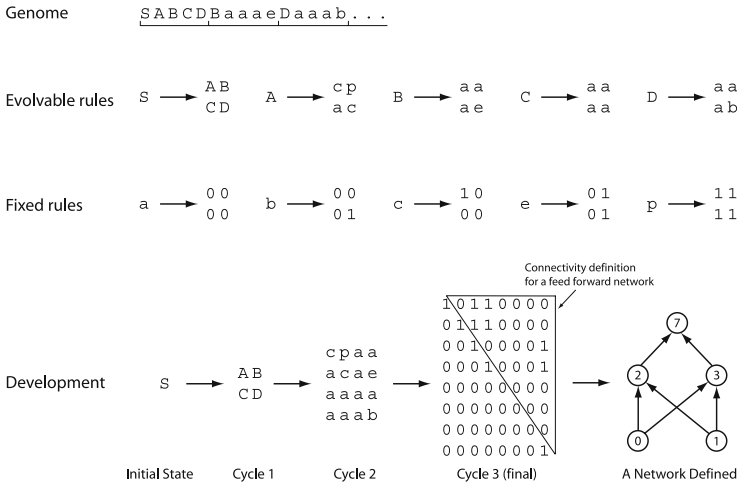
\includegraphics[width=\linewidth]{figs/kitano.png}\\
    \tiny{D. Floreano, P. D\"urr, C. Mattiussi. \textit{Neuroevolution: from architectures to learning}. Evolutionary Intelligence, Vol. 1, No. 1, pags. 47-62. Springer-Verlag. 2008.}
	\end{center}
\end{frame}

\begin{frame}[plain]{Indirect codification}{Kitano's method (III)}
	\begin{center}
	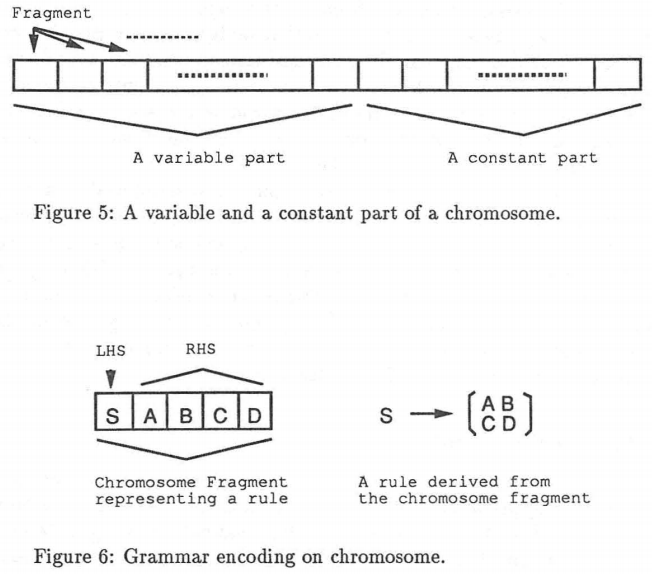
\includegraphics[width=0.7\linewidth]{figs/kitanoCodification.png}\\
    \tiny{H. Kitano. \textit{Designing Neural Networks Using Genetic Algorithms with Graph Generation System}. Complex Systems 4: 461-476. 1990.}
	\end{center}
\end{frame}


			
\end{document}
